\documentclass[a4paper, 11pt]{article}


\usepackage[czech]{babel}
\usepackage[utf8]{inputenc}
\usepackage[left=2cm, top=3cm, text={17cm, 24cm}]{geometry}
\usepackage{times}
\usepackage{verbatim}
\usepackage{enumitem}
\usepackage{graphicx}
\usepackage{pdflscape}
\usepackage[unicode]{hyperref}
\usepackage[table,xcdraw]{xcolor}
\usepackage{upgreek}
\usepackage{color}
\usepackage{tabularray}
\usepackage{multicol}
\usepackage{makecell}
\usepackage{tabularx}


\parskip=0.2\baselineskip % nastavuje velikost vertikální mezery mezi odstavci
\newcommand{\cunder}{\underline{\hspace{8mm}}}

\hypersetup{
    colorlinks=true,
    linkcolor=red,
    urlcolor=blue, 
    citecolor=brown
}



\begin{document}
\begin{titlepage}
		\begin{center}
			
\includegraphics[width=0.77\linewidth]{include/FIT_logo.pdf} \\

			\vspace{\stretch{0.382}}

			\Huge{Projektová dokumentace} \\
			\LARGE{\textbf{Implementace překladače jazyka IFJ23}} \\
			\Large{Tým xhalam16, varianta TRP-izp}
			\vspace{\stretch{0.618}}
		\end{center}

		\begin{minipage}{0.4 \textwidth}
			{\Large \today}
		\end{minipage}
		\hfill
		\begin{minipage}[r]{0.6 \textwidth}
			\Large
			\begin{tabular}{l l l}
				\textbf{Marek Halamka} & \textbf{(xhalam16)} & \quad 45\,\% \\
				Šimon Motl & (xmotls00) & \quad 35\,\% \\
				Richard Juřica & (xjuric31) & \quad 20\,\% \\
				Jan Kroutil & (xkrout04) & \quad 0\,\% \\
			\end{tabular}
		\end{minipage}
	\end{titlepage}
	\thispagestyle{empty}

	{\hypersetup{
		linkcolor=black,
	}
	\tableofcontents
	}

	\newpage
	\setcounter{page}{1}
	\section{Úvod}
	Překladač jazyka IFJ23 je projekt vytvořený v~rámci předmětů IFJ a IAL na FIT VUT v~Brně. 
	\par\noindent Cílem projektu je vytvořit překladač jazyka IFJ23, který bude překládat zdrojový kód napsaný v~tomto jazyce do cílového jazyka IFJcode23 a vrací příslušný návratový kód.
	\par\noindent Program je implementován jako konzolová aplikace, která na standardní vstup přijímá zdrojový kód jazyka IFJ23 a na standardní výstup vypisuje cílový kód jazyka IFJcode23. 
	\par\noindent Překladač je implementován v~jazyce C dle normy C11\footnote{ISO/IEC 9899:2011, viz. \url{https://www.iso.org/standard/57853.html}} a je rozdělen do několika modulů. Každý modul má svůj hlavičkový soubor, který obsahuje deklarace funkcí a struktur definovaných v~daném modulu. 


	\section{Implementace}
	Zvolená metoda implementace je jednoprůchodový \textbf{syntaxí řízený překlad} a skládá se z~částí, které jsou popsány v~následujících podkapitolách.

	\subsection{Pomocné moduly a rozhraní}
	Program mimo hlavní funkce obsahuje několik důležitých modulů a rozhraní využívaných v~rámci celého projektu. Jejich výčet a popis se nachází v~následujících podkapitolách.
	\subsubsection{Error}
	Toto rozhraní, definované v~hlavičkovém souboru \texttt{error.h}, obsahuje výčtový typ chybových stavů, které mohou nastat při běhu programu.


	\subsubsection{DynamicBuffer}
	Tento modul definovaný v~souboru \texttt{dynamic\_buffer.c} má za úkol uchovávat řetězce proměnné délky.
	Korespondující hlavičkový soubor \texttt{dynamic\_buffer.h} obsahuje deklarace funkcí a struktur definovaných v~tomto modulu.
	\par\noindent Rozhraní obsahuje strukturu \texttt{dynamic\_buffer}, která obsahuje \textbf{ukazatel} na alokovanou paměť, \textbf{kapacitu} alokované paměti a \textbf{velikost} obsazené paměti.
	\par\noindent Modul obsahuje funkce pro inicializaci, uvolnění, realokaci a práci s~řetězci. Buffer se v~případě naplění automaticky realokuje na dvojnásobek své původní kapacity.
	\par\noindent Pomocí výše zmíněných funkcí jsme definovali abstraktní datový typ \texttt{DynamicBuffer}, který je využíván v~dalších částech projektu.


	\subsubsection{DynamicArray}
	Na stejném principu jako \texttt{DynamicBuffer} je implementován i ADT \texttt{DynamicArray}, který je definován v~souboru \texttt{dynamic\_array.c} s~rozhraním v~souboru \texttt{dynamic\_array.h}.
	\par\noindent Struktura definující tento typ obsahuje \textbf{ukazatel} na alokovanou paměť, \textbf{kapacitu} alokované paměti a \textbf{velikost} obsazené paměti. Pole uchovává proměnný počet struktury typu \texttt{ArrayItem}, které obsahují ukazatel na typ \texttt{void}. Tím jsme docílili toho, že do pole můžeme ukládat jakýkoliv typ dat.
	\par\noindent Používá se především v~generování cílového kódu, více o~tom v~sekci \ref{sec:gen}.

	\newpage
	\subsubsection{Token}
	Hlavičkový soubor \texttt{token.h} obsahuje definici struktury \texttt{token}, která reprezentuje token.
	\par\noindent Struktura obsahuje typ tokenu, hodnotu tokenu a textovou reprezentaci tokenu ve zdrojovém souboru. 
	\par\noindent \textbf{Typ tokenu} je definován výčtovým typem \texttt{token\_type}, který obsahuje všechny typy tokenů jazyka IFJ23. Může nabývat i speciálních hodnot jako \texttt{TOKEN\_UNKNOWN} signalizující lexikální chybu, \texttt{TOKEN\_ERROR}, který dává najevo výskyt nějaké interní chyby, \texttt{TOKEN\_EOF} a \texttt{TOKEN\_NONE} použitý pro komentáře.
	\par\noindent \textbf{Hodnota tokenu} je typu \texttt{union}, a nabývá buď hodnoty odpovídající číslené hodnotě tokenu, nebo ukazatele na dříve definovanou strukturu \texttt{DynamicBuffer}, která reprezentuje řetězec.
	Typ union byl zvolen z~důvodu úspory paměti, protože token může obsahovat pouze jednu z~těchto hodnot.
	\par\noindent \textbf{Textová reprezentace tokenu} ve zdrojovém souboru je uložena jako ukazatel na strukturu \texttt{DynamicBuffer}, který obsahuje řetězec.
	Je uchovávána z~důvodu implementace funkce \texttt{peek\_token}, která je podrobněji popsána v~sekci \ref{sec:lex}.

	\subsubsection{Tabulka symbolů}
	Tabulka symbolů slouží k~uložení informací o~proměnných a funkcích.
	\par\noindent Deklarace proměnné či funkce odpovídá vytvoření záznamu v~tabulce symbolů, kde klíčem je \textbf{identifikátor} proměnné.
	\par\noindent Dle zvolené varianty zadání je tabulka symbolů implementována jako \textbf{TRP s~otevřenou adresací}.
	\par\noindent Implicitní rozptýlení využívá \textbf{lineární} určení kroku při výpočtu dalšího volného indexu. 
	\par\noindent Tabulka symbolů je implementována v~souboru \texttt{symtable.c} s~rozhraním v~souboru \texttt{symtable.h}.
	\par\noindent Rozhraní obsahuje funkce pro inicializaci, uvolnění, vložení a vyhledání položky v~tabulce symbolů či vytvoření nové položky.
	\par\noindent Kromě těchto funkcí obsahuje i signaturní \textbf{hashovací funkci}, která je použita při transformaci klíče, na index do tabulky symbolů.
	\begin{figure}[h]
		\centering
		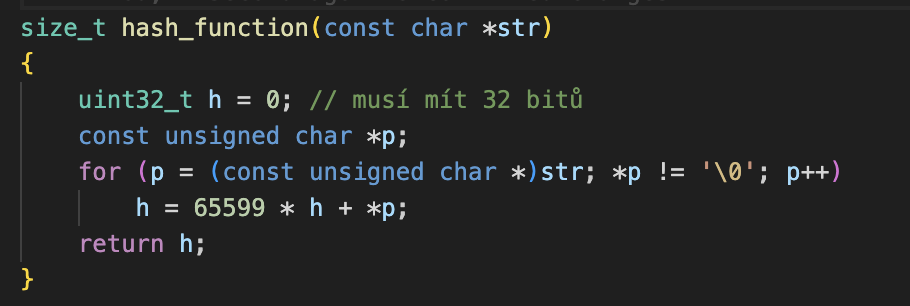
\includegraphics[width=0.5\linewidth]{include/hash_function.png}
		\caption{Hashovací funkce}
		\label{fig:hash_function}
	\end{figure}

	\par\noindent Při vytváření hashovací funkce jsme čerpali informace z~předmětů IJC, IAL a zde: \cite{HASH_FUNC}.


	\par\noindent Tabulka se v~případě naplnění automaticky \textbf{realokuje} na dvojnásobek své původní kapacity.
	\par\noindent V~programu rozlišujeme mezi \texttt{GLOBÁLNÍ} a \texttt{LOKÁLNÍ} tabulkou symbolů. Globální tabulka symbolů je vytvořena při inicializaci programu a je uvolněna při jeho ukončení. Lokální tabulka symbolů je vytvořena při vstupu do bloku a je uvolněna při jeho opuštění.
	\par\noindent Tyto typy tabulek se liší mimojiné i v~datech, které uchovávají. Funkce pro práci s~tabulkou symbolů jsou implementovány tak, aby bylo možné používat stejné funkce pro oba typy tabulek. Docíleno je to pomocí ukazatele typu \texttt{void}, který je přetypován na konkrétní typ tabulky symbolů v~závislosti na tom, zda se jedná o~\texttt{GLOBÁLNÍ} nebo \texttt{LOKÁLNÍ} tabulku symbolů.
	


	\subsubsection{Parameter list}
	Parametry funkcí jsou uchovávány v~seznamu, který je implementován jako \textbf{jednosměrně vázaný seznam}.
	\par\noindent Seznam je implementován v~souboru \texttt{symtable.c} s~rozhraním v~souboru \texttt{symtable.h}.
	\par\noindent Rozhraní obsahuje funkce pro inicializaci, uvolnění, vložení a vyhledání položky v~seznamu.
	\par\noindent Implementací výše zmíněných funkcí je definován abstraktní datový typ \texttt{parameter\_list\_t}, který je vy\-užíván v~dalších částech projektu.


	\subsubsection{Stack}
	Zásobník je v~projektu využíván na více místech, pokaždé pro ukládání jiného typu dat.
	\par\noindent Proto byl zásobník implementován jako \textbf{obecný zásobník}, který je definován v~souboru \texttt{stack.c} s~rozhraním v~souboru \texttt{stack.h}.
	\par\noindent Zásobník uchovává položky typu \texttt{Stack\_Frame}, které obsahují ukazatel na data typu \texttt{void}. Tím je umožněno ukládat na zásobník jakýkoliv typ dat.
	\par\noindent Rozhraní obsahuje známé funkce pro práci se zásobníkem. Tím je definován abstraktní datový typ \texttt{Stack}.
	\par\noindent Za účelem ulehčení řešení některých problémů, které se vyskytly při implementaci, rozhraní zásobníku poskytuje i funkci \texttt{Stack\_get(stack,index)}, která vrací položku na zadaném indexu.
	\par\noindent Jelikož struktura ukládá data jako ukazatel, je potřeba dát pozor, nad čím voláme operaci \texttt{free}. Proto byla implementována funkce \texttt{stack\_empty}, která uvolní všechny ukazatele na zásobníku. Funkce předpokládá, že na zásobníku jsou pouze ukazatele na dynamicky alokovanou paměť.
	\par\noindent Pokud dojde k~naplnění zásobníku, je automaticky \textbf{realokován} na dvojnásobek své původní kapacity.

	\subsection{Lexikální analýza} \label{sec:lex}
	Lexikální analýza je definována v~souboru \texttt{scanner.c} s~rozhraním v~souboru \texttt{scanner.h} a implementována jako \textbf{deterministický konečný automat}. Graf konečného automatu je zobrazen \hyperref[sec:fa]{zde}.
	\par\noindent Automat se rozhoduje na základě aktuálního stavu a načteného znaku ze vstupního souboru.
	\par\noindent V~jazyce C je implementován pomocí konstrukce \texttt{if...else if}, kde každá větev odpovídá jednomu stavu automatu. Automat také využívá a nastavuje pomocné statické globální proměnné, které jsou definovány v~souboru \texttt{scanner.h}. 
	\par\noindent Hlavní funkce, kterou analýza implementuje je \texttt{get\_token}, která vrací dříve popsaný \texttt{token} načtený ze vstupního souboru. Postupně načítá znaky ze vstupního souboru a předává je automatu, který na základě aktuálního stavu a načteného znaku rozhodne o~dalším postupu. Pokud načtený znak neodpovídá žádnému stavu, vrátí funkce token s~typem \texttt{TOKEN\_UNKNOWN}, který signalizuje lexikální chybu.
	Načtené znaky jsou ukládány do datového typu \texttt{DynamicBuffer}, který automat postupně kontroluje, zda neodpovída některému z~klíčových slov jazyka IFJ23. Pokud ano, je vrácen token s~odpovídajícím typem klíčového slova.
	\par\noindent Je-li některý z~načtených tokenů typu číslo nebo řetězec, je do unie \texttt{token\_value} uložena i korespondující hodnota tohoto tokenu. Pokud se jedná o~desetinné číslo typu Double zadané ve speciální notaci, jako např. \texttt{1.0e-10}, je hodnota scannerem převedena na desetinné číslo. Podobně je to tak i u~řetězců obsahující escape sekvence, které jsou převedeny na odpovídající znaky.
	\par\noindent Scanner také implementuje funkci \texttt{peek\_token}, která vrací následující token ze vstupního souboru, ale nečte ho. Tato funkce je využívána v~syntaktické analýze pro predikci následujícího tokenu. Pro implementaci této funkce byla za potřebí implementovat pomocná funkce \texttt{unget\_token}, která vrátí znaky uložené v~\texttt{DynamicBuffer} zpět do vstupního souboru.


	
	\subsection{Syntaktická analýza}
	Jelikož je překladač implementován pomocí metody syntaxí řízeného překladu, je syntaktická analýza nej\-důležitější částí celého projektu.
	Je implementována v~souboru \texttt{parser.c} s~rozhraním v~souboru \texttt{parser.h}. Toto rozhraní poskytuje funkci \texttt{parse}, která je volána z~hlavní funkce programu.
	\par\noindent Syntaktická analýza se řídí LL -- gramatikou předem definovanou pro jazyk IFJ23, zobrazenou \hyperref[sec:ll_grammar]{zde}. Využívá metodiky \textbf{rekurzivního sestupu} podle pravidel v~LL -- tabulce, kterou můžete nalézt \hyperref[sec:ll_table]{zde}.
	Dále využívá metodu \textbf{precedenční syntaktické analýzy} pro zpracování výrazů, více o~této metodě v~sekci \ref{sec:precedence}.
	\par\noindent Po dobu syntaktické analýzy je volána funkce \texttt{get\_token} z~modulu \texttt{scanner}. Na základě typu vráceného tokenu se rozhoduje o~syntaktické validitě zdrojového kódu. Funkce \texttt{parse} si volá pomocné funkce podle typu neterminálu na pravé straně aplikovaného pravidla.

	\subsubsection{Syntaktický strom}
	Definici struktury \texttt{TreeNode}, reprezentující uzel syntaktického stromu, najdeme v~rozhraní. Tato struktura obsahuje typ uzlu, který je definován výčtovým typem \texttt{node\_type} a pole proměnné délky ukazatelů na potomky uzlu. 
	Dále uzel může uchovávát informace o~tokenech, jako například hodnotu konstanty nebo název identifikátoru proměnné či funkce.
	\par\noindent Při aplikování pravidel LL -- gramatiky jsou vytvářeny uzly syntaktického stromu nebo v~případě neúspěchu při aplikování některého z~pravidel je signalizována syntaktická chyba a program je ukončen.
	Pro tvorbu stromu jsme využili datovou strukturu \textbf{obecného stromu}, který je zakořeněn v~uzlu \texttt{root} s~typem \texttt{NODE\_PROGRAM} a tvoří se \textbf{shora dolů}.
	\par\noindent Při tvorbě stromu jsou jednotlivé podstromy postupně kontrolovány sémantickou analýzou a následně generován cílový kód. Bližší popis volání sémantic\-kých akcí je zde \ref{sec:sem}.
	\subsubsection{Práce s~tabulkami symbolů}
	Parser se stará o~vytvoření a naplnění tabulek symbolů. V~jazyce IFJ23 existují dva typy tabulek symbolů, \texttt{GLOBÁLNÍ} a \texttt{LOKÁLNÍ}.
	Globální tabulka je právě jedna a je vytvořena při inicializaci programu. Do globální tabulky jsou ukládány informace o~funkcích a globálních proměnných.
	\par\noindent Lokální tabulka symbolů je vytvářena při vstupu do bloku a je uvolněna při jeho opuštění. Do lokální tabulky jsou ukládány informace o~lokálních proměnných.
	\par\noindent Syntaktická analýza také vytváří zásobník lokálních tabulek symbolů, který je využíván sémantickými akcemi. Parser zajišťuje správné přidání a odebírání lokálních tabulek symbolů ze zásobníku. 

	\subsubsection{Zpracování výrazů pomocí precedenční syntaktické analýzy}
	\label{sec:precedence}
	Postup zpracování výrazů je založen na precedenční tabulce, kterou naleznete \hyperref[sec:precedence_table]{zde}. V~jazyce C byla implementována jako dvourozměrné pole znaků, kde každý typ znak určuje akci, která se má dál provést. 
	\par\noindent K~implementaci analýzy byl využit dříve definovaný ADT \texttt{Stack}. Výrazy jsou zpracovávány \textbf{zdola nahoru} a výsledný strom je vytvářen \textbf{shora dolů}. K~tomu je využit další zásobík \texttt{Stack}, kam se ukládájí jednotlivá pravidla LL -- gramatiky.


	\subsubsection{Volání sémantických akcí a generování cílového kódu}
	\label{sec:sem}
	Sémantické akce jsou volány při vytváření syntaktického stromu. Parser volá funkci \texttt{semantic} z~modulu \texttt{semantic.c} s~rozhraním v~souboru \texttt{semantic.h}. Tato funkce přijímá ukazatel na uzel syntaktického stromu a ukazatel na zásobník lokálních tabulek symbolů.
	Na základě výsledku sémantické analýzy je vygenerován cílový kód. V~případě, že došlo k~chybě, je program ukončen s~odpovídajícím návratovým kódem.


	\subsection{Sémantická analýza}
	Sémantická analýza je implementována v~souboru \texttt{semantic.c} s~rozhraním v~souboru \texttt{semantic.h}. Toto rozhraní poskytuje funkci \texttt{semantic}, která je volána z~hlavní funkce programu. Jelikož naše implementace využívá jednoprůchodový překlad, je sémantická analýza prováděna při vytváření syntaktického stromu.
	\par\noindent Ve funkci \texttt{semantic} se rozhodne, jaká sémantická akce se má provést na základě typu uzlu syntaktického stromu a zavolá se příslušná pomocná funkce. Jednotlivé funkce poté navigují v~syntaktickém stromu podle předem stanovených pravidel a provádí sémantickou kontrolu. Pokud nastane chyba, vrátí funkce odpovídající chybový kód.
	\par\noindent Sémanticka analýza ke kontrole využívá naplněné tabulky symbolů a zásobník lokálních tabulek symbolů předaný z~parseru.
	\subsubsection{Hledání v~tabulkách symbolů}
	Vždy když sémantická analýza potřebuje vyhledat položku, začne od lokální tabulky symbolů na vrcholu zásobníku lokálních tabulek symbolů a postupně se prochází všechny tabulky symbolů na zásobníku. V~případě, že položka není nalezena ani v~jedné z~tabulek na zásobníku, podívá se sémantika do globální tabulky symbolů.
	Pokud položka není nalezena ani v~globální tabulce symbolů, je vrácen chybový kód.
	\par\noindent V~případě, že se jedná o~funkci, hledá sémantická analýza rovnou v~globální tabulce symbolů. 

	\subsection{Generování cílového kódu}
	\label{sec:gen}

	Generování cílového kódu je implementováno v~souboru \texttt{code\_gen.c} s~rozhraním v~souboru \texttt{code\_gen.h}. Toto rozhraní poskytuje spoustí funkcí pro generování cílového kódu, které je obvykle volány z~hlavní funkce programu. Jelikož naše implementace využívá jednoprůchodový překlad, je generování cílového kódu pro\-váděno při vytváření syntaktického stromu.
	Využívá struktur ADT \texttt{DynamicBuffer}, ADT \texttt{DynamicArray} a především ADT \texttt{Stack} pro práci s~lokálními proměnnými. 
	\subsection{Generování výrazů}
	\label{sec:gen_expr}
	Je implementováno pomocí rekurzivního volání funkce \texttt{generateExpression}, která příjmá ukazatel na uzel syntaktického stromu, na zákldě jehož struktury se rozhoduje, jaká akce se má provést.
	\par\noindent Klíčovým faktorem při generování je vlastnost předáného uzlu, a to konkrétně počet jeho potomků. Relační operátory, které se nenachází v~instrukční sadě cílového jazyka \texttt{IFJcode23}, jsou převedeny na ekvivalentní operátory, které se v~instrukční sadě nachází.
	\subsection{Generování vestavěných funkcí}
	\label{sec:gen_builtin}
	Každá vestavěná funkce má svou vlastní funkci pro generování kódu, která na základě informací o~funkci vygeneruje odpovídající instrukci z~instrukční sady cílového jazyka \texttt{IFJcode23}. \\Výjimkou je funkce \texttt{substring}, která nemá v~instrukční sadě ekvivalentní instrukci. Proto je tato funkce implementována na základě známých algoritmů pro hledání v~řetězcích.

	\newpage
	\section{Práce v~týmu}

	\subsection{Komunikace a verzovací systém}
	V~týmu jsme komunikovali buď osobně, nebo vzdáleně pomocí aplikace Discord. Na této platformě jsme si vytvořili vlastní server, kde jsme si vytvořili kanály pro komunikaci a sdílení souborů. 
	\par\noindent Pro verzování projektu jsme zvolili verzovací systém Git se správou repozitářů pomocí služby GitHub. Náš repozitář je dostupný na adrese \url{https://github.com/xhalam16/IFJ-projekt}.


	\subsection{Prvotní rozdělení práce}
	Prvotní rozdělení bylo domluveno všemi členy týmu následovně:
	\begin{itemize}
		\item \textbf{Marek Halamka} -- Lexikální analýza, tabulky symbolů  -- 25\,\%
		\item Šimon Motl -- Syntaktická analýza -- 25\,\%
		\item Richard Juřica -- Sémantická analýza -- 25\,\%
		\item Jan Kroutil -- Generování cílového kódu -- 25\,\% 
		\item Společně -- ADT Stack, ADT DynamicBuffer, ADT DynamicArray, dokumentace
	\end{itemize}

	\subsection{Finální rozdělení práce}
	Ovšem kvůli nerovnoměrné práci na projektu některých členů týmu muselo být rozdělení práce změněno na: \\
	\begin{table}[ht]
		\centering
		\renewcommand{\arraystretch}{1.3}
		\begin{tabular}{|l|l|l|}
			\hline
			\textbf{Člen} & \begin{tabular}{l} \textbf{Implementované části} \end{tabular} & \textbf{Body} \\ \hline
			\textbf{Marek Halamka} & \begin{tabular}{l} Lexikální analýza, ADT Stack a ADT DynamicBuffer,\\ tabulky symbolů, sémantická analýza, dokumentace \end{tabular} & 45\,\% \\ \hline
			Šimon Motl & \begin{tabular}{l} Syntaktická analýza, generování kódu, ADT DynamicArray, dokumentace \end{tabular} & 35\,\% \\ \hline
			Richard Juřica & \begin{tabular}{l} Generování kódu \end{tabular} & 20\,\% \\ \hline
			Jan Kroutil &  & 0\,\% \\ \hline
		\end{tabular}
		\caption{Finální rozdělení práce}
	\end{table}

	\subsection{Zdůvodnění odchylek od rovnoměrného rozdělení}
	Někteří členové týmu se neúčastnili na projektu vůbec, nebo se účastnili minimálně. Proto bylo nutné práci rozdělit mezi zbylé členy týmu, aby se projekt stihl včas dokončit. 
	To vedlo k~nerovnoměrnému rozdělení práce (viz. tabulka výše) a tím pádem i k~nerovnoměrnému rozdělení bodů.

	\newpage
	\section{Závěr}
	Díky projektu jsme se naučili pracovat v~týmu a využívat verzovací systém Git. Dále jsme si osvojili znalosti o~tom jak překladač funguje a jaké fáze překladu musí projít zdrojový kód, než je spuštěn.
	\par\noindent I~přes některé komplikace, které jsme museli řešit, jsme s~výsledkem spokojeni. Jsme si vědomi, že některé části projektu jsme mohli implementovat lépe, ale vzhledem k~časové tísni jsme se rozhodli, že je lepší projekt dokončit včas, než se zdržovat a riskovat, že projekt nestihneme včas dokončit.
	\par\noindent Naše řešení se místy může trošku odchýlit od oficiálních materiálů, převážně z~důvodu, že jsme s~implementací začali s~předstihem než byla témata detailně vysvětlena, ale \textbf{závazné metody} jsme samozřejmě \textbf{dodrželi}.
	

	\newpage
	\bibliographystyle{czechiso}
	\renewcommand{\refname}{Literatura}
	\bibliography{dokumentace}



	\newpage
	\section*{Precedenční tabulka}
	\label{sec:precedence_table}
	\addcontentsline{toc}{section}{Precedenční tabulka}
\begin{table}[h]
	\centering
	\resizebox{0.7\linewidth}{!}{
	\begin{tabular}{|
	>{\columncolor[HTML]{9CC2E5}}c |c|c|c|c|c|c|c|c|}
	\hline
	\multicolumn{1}{|l|}{\cellcolor[HTML]{9CC2E5}{\color[HTML]{FFFFFF} }} & \cellcolor[HTML]{9CC2E5}\textbf{2} & \cellcolor[HTML]{9CC2E5}\textbf{1} & \cellcolor[HTML]{9CC2E5}\textbf{(} & \cellcolor[HTML]{9CC2E5}\textbf{)} & \cellcolor[HTML]{9CC2E5}\textbf{id} & \cellcolor[HTML]{9CC2E5}\textbf{0} & \cellcolor[HTML]{9CC2E5}\textbf{4} & \cellcolor[HTML]{9CC2E5}\textbf{END} \\ \hline
	\textbf{2}                                                            & \textgreater{}                     & \textless{}                        & \textless{}                        & \textgreater{}                     & \textless{}                         & \textless{}                        & \textgreater{}                     & \textgreater{}                       \\ \hline
	\textbf{1}                                                            & \textgreater{}                     & \textgreater{}                     & \textless{}                        & \textgreater{}                     & \textless{}                         & \textless{}                        & \textgreater{}                     & \textgreater{}                       \\ \hline
	\textbf{(}                                                            & \textless{}                        & \textless{}                        & \textless{}                        & =                                  & \textless{}                         & \textless{}                        & \textless{}                        &                                      \\ \hline
	\textbf{)}                                                            & \textgreater{}                     & \textgreater{}                     &                                    & \textgreater{}                     &                                     & \textgreater{}                     & \textgreater{}                     & \textgreater{}                       \\ \hline
	\textbf{id}                                                           & \textgreater{}                     & \textgreater{}                     &                                    & \textgreater{}                     &                                     & \textgreater{}                     & \textgreater{}                     & \textgreater{}                       \\ \hline
	\textbf{0}                                                            & \textgreater{}                     & \textgreater{}                     &                                    & \textgreater{}                     &                                     & \textgreater{}                     & \textgreater{}                     & \textgreater{}                       \\ \hline
	\textbf{4}                                                            & \textless{}                        & \textless{}                        & \textless{}                        & \textgreater{}                     & \textless{}                         & \textless{}                        & \textless{}                        & \textgreater{}                       \\ \hline
	\textbf{END}                                                          & \textless{}                        & \textless{}                        & \textless{}                        &                                    & \textless{}                         & \textless{}                        & \textless{}                        &                                      \\ \hline
	\end{tabular}
	}
	\caption{Precedenční tabulka}
	\label{tab:precedence_table}
	\end{table}

	Vysvětlivky k~tabulce:
	\begin{itemize}
		\item \textbf{0} -- Operátor s~prioritou 0, tedy \texttt{!}
		\item \textbf{1} -- Operátor s~prioritou 1, tedy \texttt{*} a \texttt{/}
		\item \textbf{2} -- Operátor s~prioritou 2, tedy \texttt{+} a \texttt{-}
		\item \textbf{3} -- Operátor s~prioritou 3, tedy \texttt{<}, \texttt{<=}, \texttt{>}, \texttt{>=}, \texttt{==} a \texttt{!=}
		\item \textbf{4} -- Operátor s~prioritou 4, tedy \texttt{??}
		\item \textbf{id} -- Identifikátor
		\item \textbf{END} -- Konec výrazu
	\end{itemize}


	\newpage
	\section*{LL -- gramatika}
	\addcontentsline{toc}{section}{LL -- gramatika}
	\label{sec:ll_grammar}
	{ \fontsize{10}{12}\selectfont 
	\begin{enumerate}[noitemsep]
		
		\item \texttt{<program> $\rightarrow$ <command> EOL <program>}
		\item \texttt{<program> $\rightarrow$ EOF}
		\item \texttt{<command> $\rightarrow\,\,\upvarepsilon$}
		\item \texttt{<command> $\rightarrow$ <assign>}
		\item \texttt{<command> $\rightarrow$ <declaration>}
		\item \texttt{<command> $\rightarrow$ <func\_declaration>}
		\item \texttt{<command> $\rightarrow$ <if\_statement>}
		\item \texttt{<command> $\rightarrow$ <while>}
		\item \texttt{<command> $\rightarrow$ <func\_call>}
		\item \texttt{<assign> $\rightarrow$ <left\_value> = <right\_value>}
		\item \texttt{<left\_value> $\rightarrow$ identifier}
		\item \texttt{<left\_value> $\rightarrow$ <declaration>}
		\item \texttt{<left\_value> $\rightarrow$ <declaration\_keyword> identifier}
		\item \texttt{<right\_value> $\rightarrow$ <expression>}
		\item \texttt{<right\_value> $\rightarrow$ <func\_call>}
		\item \texttt{<declaration> $\rightarrow$ <declaration\_keyword> identifier : <datatype>}
		\item \texttt{<declaration\_keyword> $\rightarrow$ let}
		\item \texttt{<declaration\_keyword> $\rightarrow$ var}
		\item \texttt{<datatype> $\rightarrow$ INT}
		\item \texttt{<datatype> $\rightarrow$ DOUBLE}
		\item \texttt{<datatype> $\rightarrow$ STRING}
		\item \texttt{<datatype> $\rightarrow$ INT?}
		\item \texttt{<datatype> $\rightarrow$ DOUBLE?}
		\item \texttt{<datatype> $\rightarrow$ STRING?}
		\item \texttt{<value> $\rightarrow$ identifier}
		\item \texttt{<value> $\rightarrow$ int}
		\item \texttt{<value> $\rightarrow$ double}
		\item \texttt{<value> $\rightarrow$ string}
		\item \texttt{<value> $\rightarrow$ nil}
		\item \texttt{<func\_call> $\rightarrow$ identifier ( <param\_list1> ) }
        \item \texttt{<param\_list1> $\rightarrow$ <param> <param\_list1\_next> }
		\item \texttt{<param\_list1> $\rightarrow$ $\upvarepsilon$}
		\item \texttt{<param\_list1\_next> $\rightarrow$ , <param> <param\_list1\_next>}
        \item \texttt{<param\_list1\_next> $\rightarrow$ $\upvarepsilon$}
		\item \texttt{<param> $\rightarrow$ <value>}
		\item \texttt{<param> $\rightarrow$ identifier : <value>}
		\item \texttt{<func\_declaration> $\rightarrow$ func identifier ( <label> identifier : <datatype> \\ <param\_list0> <return\_type> \{ EOL <body> }
		\item \texttt{<return\_type>  $\rightarrow\,\,\upvarepsilon$}
		\item \texttt{<return\_type>  $\rightarrow$ -> <datatype>}
		\item \texttt{<param\_list0>  $\rightarrow$ )}
		\item \texttt{<param\_list0>  $\rightarrow$ , <label> identifier : <datatype> <param\_list0>}
		\item \texttt{<label>  $\rightarrow$ \rule{3mm}{.5pt}}
		\item \texttt{<label>  $\rightarrow$ identifier}
		\item \texttt{<body>  $\rightarrow$ <command> EOL <body>}
		\item \texttt{<body>  $\rightarrow$ return <return\_value> EOL <body>}
		\item \texttt{<body>  $\rightarrow$ \}}
		\item \texttt{<return\_value>  $\rightarrow\,\,\upvarepsilon$}
		\item \texttt{<return\_value>  $\rightarrow$ <func\_call>}
		\item \texttt{<return\_value>  $\rightarrow$ <expression>}
		\item \texttt{<if\_statement>  $\rightarrow$ if <condition>  \{ <body> else \{ <body>}
		\item \texttt{<condition> $\rightarrow$ let identifier}
		\item \texttt{<condition> $\rightarrow$ <expression>}
		\item \texttt{<while> $\rightarrow$ while <expression> \{ <body>}
		
	\end{enumerate}
	}

	\newpage
	\section*{LL -- tabulka}
	\label{sec:ll_table}
	\addcontentsline{toc}{section}{LL -- tabulka}
	

\newcommand{\gt}{\textgreater{}}
\newcommand{\lt}{\textless{}}
\newcommand{\vcen}[1]{%
    \raisebox{3.5\normalbaselineskip}[0pt][0pt]{\rotatebox[origin=c]{90}{#1}}%
}

\definecolor{RegentStBlue}{rgb}{0.611,0.76,0.898}
% \begin{landscape}
\renewcommand{\arraystretch}{1.8}
\begin{table}[!ht]
	\centering
	\Huge
	\setlength{\tabcolsep}{10pt} % Horizontal spacing
	\resizebox{1\linewidth}{!}{
    \begin{tabular}{|>{\columncolor{RegentStBlue}}c|c|c|c|c|c|c|c|c|c|c|c|c|c|c|c|c|c|c|c|c|c|c|}
    \hline
		\rowcolor{RegentStBlue}
        \textbf{} & \vcen{\textbf{\lt program \gt}} & \vcen{\textbf{\lt command \gt}} &  \vcen{\textbf{\lt assign \gt}}& \vcen{\textbf{\lt left\_value \gt}} & \vcen{\textbf{\lt right\_value \gt}} & \vcen{\textbf{\lt declaration \gt}} &  \rotatebox{90}{\textbf{\lt declaration\_keyword \gt}} & \vcen{\textbf{\lt datatype \gt}} &  \vcen{\textbf{\lt value \gt}} & \vcen{\textbf{\lt func\_call \gt}} & \vcen{\textbf{\lt param\_list1 \gt}} & \vcen{\textbf{\lt param\_list1\_next \gt}}  & \vcen{\textbf{\lt param \gt}} & \vcen{\textbf{\lt func\_declaration \gt}} &  \vcen{\textbf{\lt return\_type \gt}} & \vcen{\textbf{\lt param\_list0 \gt}} & \vcen{\textbf{\lt label \gt}} & \vcen{\textbf{\lt body \gt}} & \vcen{\textbf{\lt return\_value \gt}} & \vcen{\textbf{\lt if\_statement \gt}} &  \vcen{\textbf{\lt condition \gt}} &  \vcen{\textbf{\lt while \gt}} \\ \hline
        \textbf{epsilon} & 1 & 3 & ~ & ~ & ~ & ~ & ~ & ~ & ~ & ~ & 32 & 34 & ~ & ~ & 38 & ~ & ~ & 44 & 47 & ~ & ~ & ~   \\ \hline
        \textbf{identifier} & 1 & 4, 9 & 10 & 11 & 15 & ~ & ~ & ~ & 25 & 30 & 31 & ~ & 35, 36 & ~ & ~ & ~ & 43 & 44 & 48 & ~ & ~ & ~ \\ \hline
        \textbf{let} & 1 & 4, 5 & 10 & 12, 13 & ~ & 16 & 17 & ~ & ~ & ~ & ~ & ~ & ~ & ~ & ~ & ~ & ~ & 44 & ~ & ~ & 51 & ~  \\ \hline
        \textbf{var} & 1 & 4, 5 & 10 & 12, 13 & ~ & 16 & 18 & ~ & ~ & ~ & ~ & ~ & ~ & ~ & ~ & ~ & ~ & 44 & ~ & ~ & ~ & ~  \\ \hline
        \textbf{func} & 1 & 6 & ~ & ~ & ~ & ~ & ~ & ~ & ~ & ~ & ~ & ~ & ~ & 37 & ~ & ~ & ~ & 44 & ~ & ~ & ~ & ~  \\ \hline
        \textbf{if} & 1 & 7 & ~ & ~ & ~ & ~ & ~ & ~ & ~ & ~ & ~ & ~ & ~ & ~ & ~ & ~ & ~ & 44 & ~ & 50 & ~& ~  \\ \hline
        \textbf{while} & 1 & 8 & ~ & ~ & ~ & ~ & ~ & ~ & ~ & ~ & ~ & ~ & ~ & ~ & ~ & ~ & ~ & 44 & ~ & ~ & ~ & 53  \\ \hline
		\textbf{,} & ~ & ~ & ~ & ~ & ~ & ~ & ~ & ~ & ~ & ~ & ~ & 33 & ~ & ~ & ~ & 41 & ~ & ~ & ~ & ~ & ~ & ~  \\ \hline
        \textbf{EOF} & 2 & ~ & ~ & ~ & ~ & ~ & ~ & ~ & ~ & ~ & ~ & ~ & ~ & ~ & ~ & ~ & ~ & ~ & ~ & ~ & ~ & ~ \\ \hline
        \textbf{INT} & ~ & ~ & ~ & ~ & ~ & ~ & ~ & 19 & ~ & ~ & ~ & ~ & ~ & ~ & ~ & ~ & ~ & ~ & ~ & ~ & ~ & ~  \\ \hline
        \textbf{DOUBLE} & ~ & ~ & ~ & ~ & ~ & ~ & ~ & 20 & ~ & ~ & ~ & ~ & ~ & ~ & ~ & ~ & ~ & ~ & ~ & ~ & ~ & ~  \\ \hline
        \textbf{STRING} & ~ & ~ & ~ & ~ & ~ & ~ & ~ & 21 & ~ & ~ & ~ & ~ & ~ & ~ & ~ & ~ & ~ & ~ & ~ & ~ & ~ & ~  \\ \hline
        \textbf{INT?} & ~ & ~ & ~ & ~ & ~ & ~ & ~ & 22 & ~ & ~ & ~ & ~ & ~ & ~ & ~ & ~ & ~ & ~ & ~ & ~ & ~& ~   \\ \hline
        \textbf{DOUBLE?} & ~ & ~ & ~ & ~ & ~ & ~ & ~ & 23 & ~ & ~ & ~ & ~ & ~ & ~ & ~ & ~ & ~ & ~ & ~ & ~ & ~ & ~  \\ \hline
        \textbf{STRING?} & ~ & ~ & ~ & ~ & ~ & ~ & ~ & 24 & ~ & ~ & ~ & ~ & ~ & ~ & ~ & ~ & ~ & ~ & ~ & ~ & ~ & ~  \\ \hline
        \textbf{int} & ~ & ~ & ~ & ~ & ~ & ~ & ~ & ~ & 26 & ~ & 31 & ~ & 35 & ~ & ~ & ~ & ~ & ~ & ~ & ~ & ~ & ~  \\ \hline
        \textbf{double} & ~ & ~ & ~ & ~ & ~ & ~ & ~ &  & 27 & ~ & 31 & ~ & 35 & ~ & ~ & ~ & ~ & ~ & ~ & ~ & ~ & ~   \\ \hline
        \textbf{string} & ~ & ~ & ~ & ~ & ~ & ~ & ~ & ~ & 28 & ~ & 31 & ~ & 35 & ~ & ~ & ~ & ~ & ~ & ~ & ~ & ~ & ~  \\ \hline
        \textbf{nil} & ~ & ~ & ~ & ~ & ~ & ~ & ~ & ~ & 29 & ~ & 31 & ~ & 35 & ~ & ~ & ~ & ~ & ~ & ~ & ~ & ~ & ~  \\ \hline
        \textbf{)} & ~ & ~ & ~ & ~ & ~ & ~ & ~ & ~ & ~ & ~ & ~ & ~ & ~ & ~ & ~ & 40 & ~ & ~ & ~ & ~ & ~ & ~  \\ \hline
        \textbf{\cunder} & ~ & ~ & ~ & ~ & ~ & ~ & ~ & ~ & ~ & ~ & ~ & ~ & ~ & ~ & ~ & ~ & 42 & ~ & ~ & ~ & ~ & ~  \\ \hline
		\textbf{\}} & ~ & ~ & ~ & ~ & ~ & ~ & ~ & ~ & ~ & ~ & ~ & ~ & ~ & ~ & ~ & ~ & ~ & 46 & ~ & ~ & ~ & ~  \\ \hline
		\textbf{$\rightarrow$} & ~ & ~ & ~ & ~ & ~ & ~ & ~ & ~ & ~ & ~ & ~ & ~ & ~ & ~ & 39 & ~ & ~ & ~ & ~ & ~ & ~ & ~  \\ \hline
		\textbf{return} & ~ & ~ & ~ & ~ & ~ & ~ & ~ & ~ & ~ & ~ & ~ & ~ & ~ & ~ & ~ & ~ & ~ & 45 & ~ & ~ & ~ & ~  \\ \hline
    \end{tabular}
	}
	\caption{LL -- tabulka}
	\label{tab:ll_table}
\end{table}

\newpage
\section*{Konečný automat pro lexikální analýzu}
\label{sec:fa}
\addcontentsline{toc}{section}{Konečný automat pro lexikální analýzu}
\begin{figure}[!ht]
	\centering
	\vspace{-0.8cm}
	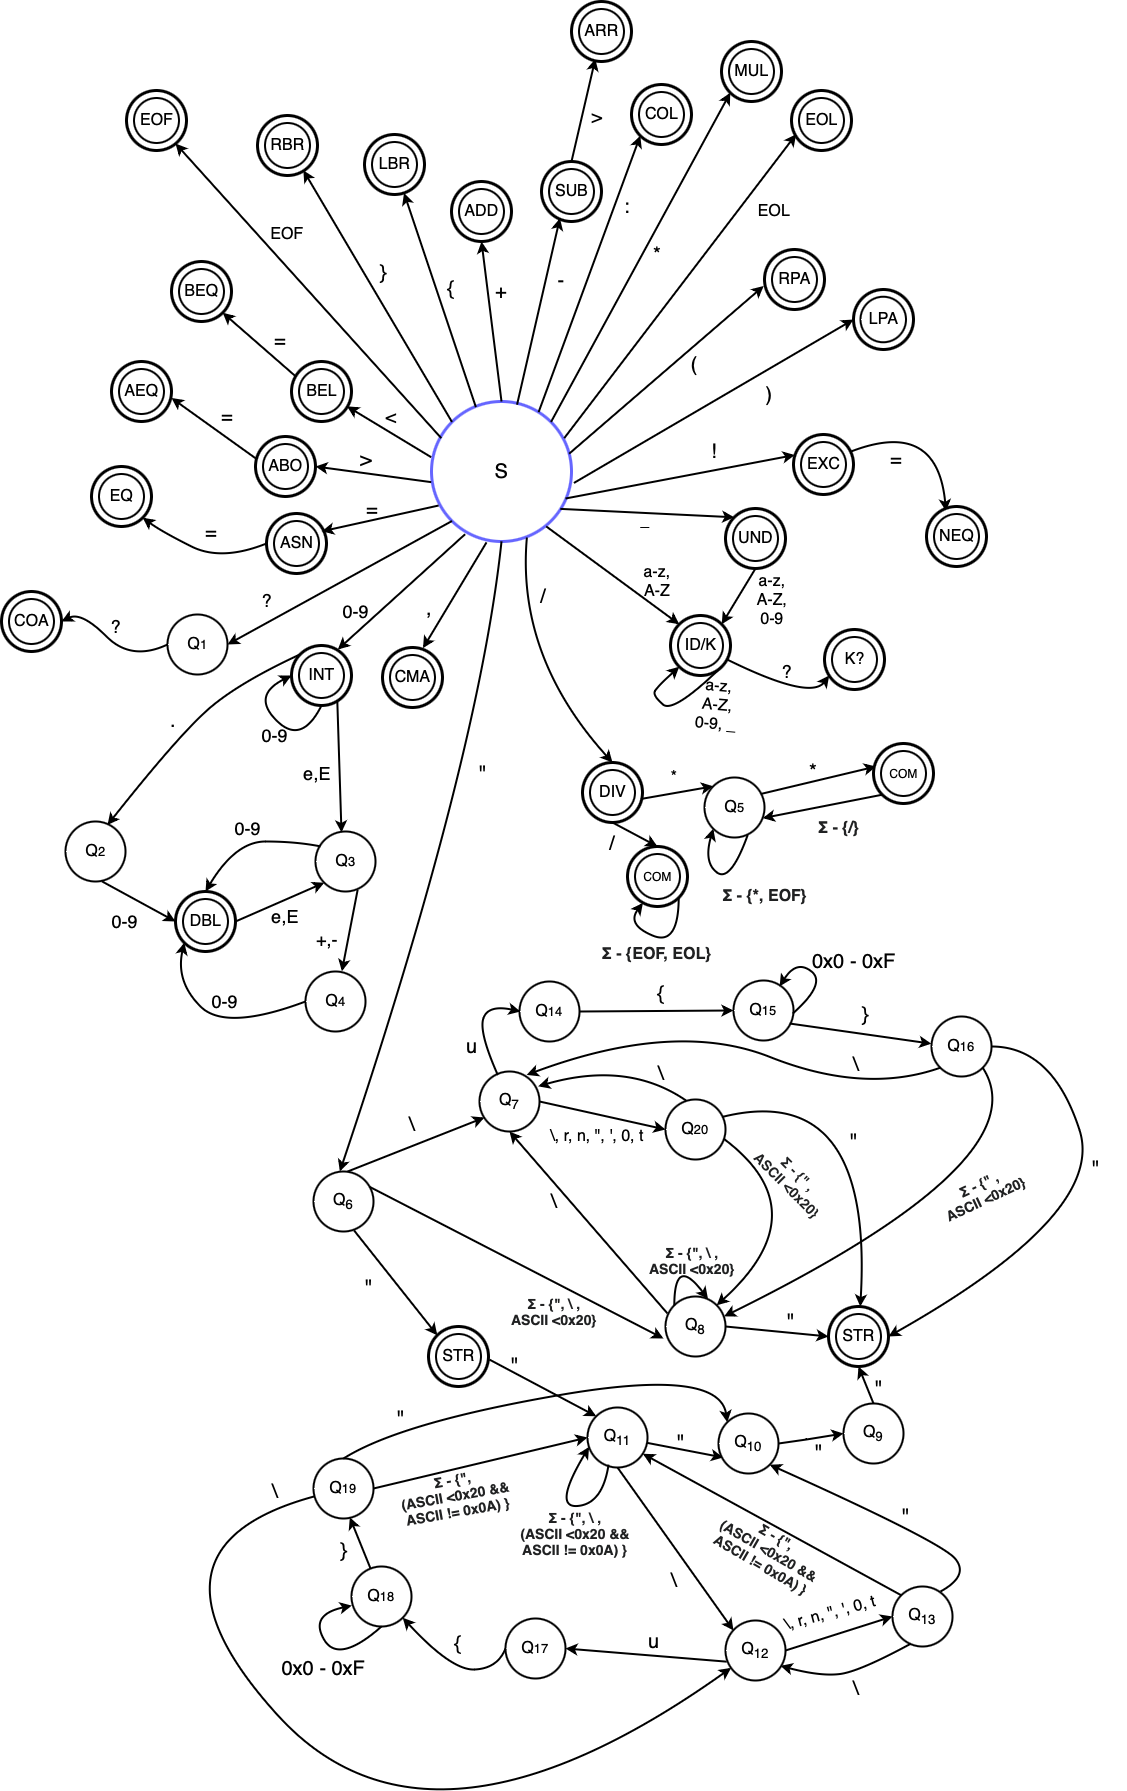
\includegraphics[width=1\linewidth, height=1.3\linewidth]{include/lex_fa.png}
	\caption{Konečný automat pro lexikální analýzu}
	\label{fig:fa}
\end{figure}



\end{document}